Keccak is an entry into the NIST SHA-3 cryptographic hash competition, and
ultimately was chosen by NIST to become SHA-3. Keccak describes a family of
cryptographic hash functions designed as a sponge construction. Bertoni et al.\
describe Keccak in \cite{bertoni2009keccak}. They build the specific variants of
Keccak on top of a permutation function called Keccak-f[b].

Variants of Keccak are primarily defined by three security parameters: the width
of the Keccak-f permutation: $b$, the capacity (the probability of success for
any generic attack against a sponge construction): $c$, and the number of rounds in
Keccak-f: $n_r$\cite{bertoni2009keccak}. The choice of these parameters has an
effect not only on the security level of the Keccak variant, but also the
performance. $r$ defines the bitrate of the sponge function, that is to say how
many bits the sponge function processes at a time, and accordingly how many
calls to the Keccak-f function are going to be made for a bitstring of a given
length. Therefore, the $r$ value is directly proportional to what we should see
as the length between upward steps in the number of cycles required to process
data.

Interestingly, the designers say that although Keccak-f is standardized on
having a width of $1600$ bits, this is optimized for a 64 bit processor. They
suggest that users of 32 bit and even embedded processors tune the function to
have a smaller width, such as $800$ to obtain better performance without totally
sacrificing security\cite{bertoni2009keccak}.

\subsubsection{keccak}
\begin{figure}[H]
    \begin{center}
        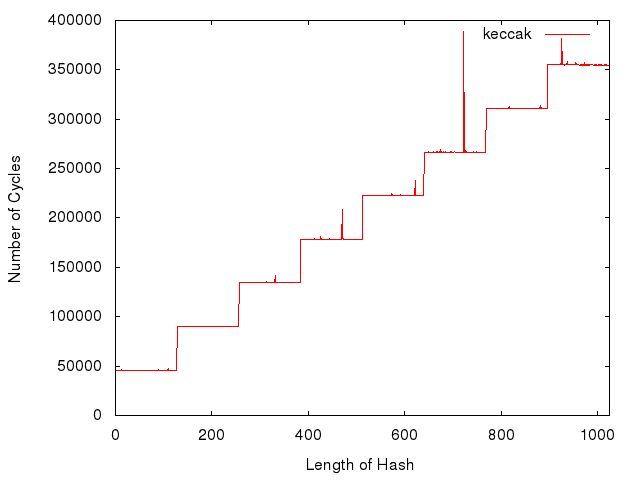
\includegraphics[scale=0.5]{images/keccak.png} 
        \caption{Keccak[]=Keccak[r=1024,c=576,nr=24] with 1024-bit output}
    \end{center}
\end{figure}

The algorithm selected to benchmark Keccak was compact, which had been compiled
with \texttt{gcc -funroll-loops -O -fomit-frame-pointer} with GCC version 4.4.5.
This version of Keccak has the parameters $ r = 1024, c = 576, n_r = 24$.

We note the stair stepped function that we associate with an additional call to
the underlying Keccak-f permutation function. We note that the steps occur every
128 bytes, which is in line with our assumption that they would be defined by
the bitrate $r = 1024$. 


\subsubsection{keccakc256}
\begin{figure}[H]
    \begin{center}
        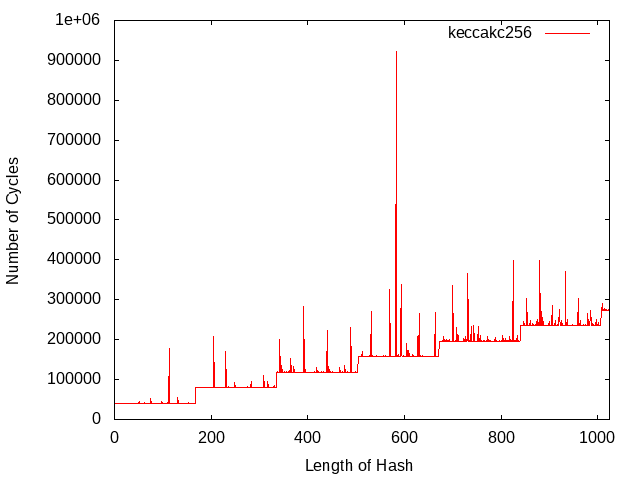
\includegraphics[scale=0.5]{images/keccakc256.png} 
        \caption{Keccak[r=1344,c=256,nr=24] with 1344-bit output}
    \end{center}
\end{figure}

The algorithm selected to benchmark Keccakc256 was compact, which had been
compiled with \texttt{gcc -mcpu=cortex-r4 -O2 -fomit-frame-pointer} with GCC
version 4.4.5. This variant of Keccak has the parameters $r=1344,c=256,n_r=24$.


This is the same implementation style as Keccak, which is unsurprising given
that all versions of Keccak are built on a similar construction. Additionally,
this version of Keccak has similar parameters to Keccak above. The longer
bit rate correctly predicts the longer period between steps on the graph when
compared to the above implementation of Keccak


\subsubsection{keccakc448}
\begin{figure}[H]
    \begin{center}
        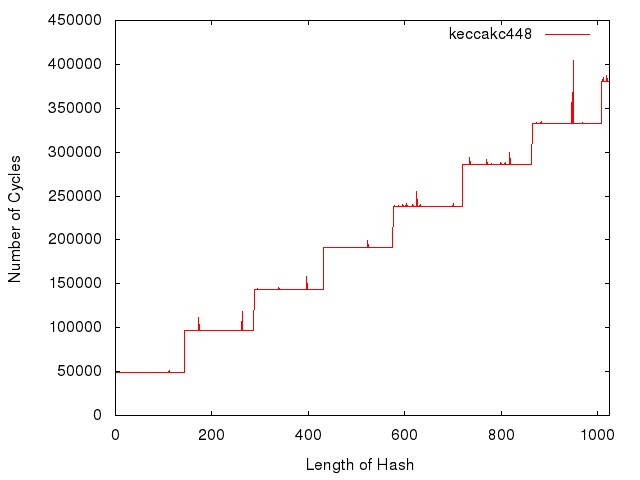
\includegraphics[scale=0.5]{images/keccakc448.png} 
        \caption{Keccak[r=1152,c=448,nr=24] with 224-bit output}
    \end{center}
\end{figure}

The algorithm selected to benchmark Keccakc448 was compact, which had been
compiled with \texttt{gcc -Os -fomit-frame-pointer} with GCC version 4.4.5. This
variant of Keccak has the parameters $r=1152,c=448,n_r=24$.

Unsurprisingly, this variant of Keccak uses the same implementation as the other
variants studied so far. This is because the Keccak family uses the same
construction internally, so optimizations from one variant for a particular
processor will work fairly well on another. 

This run shows the stair stepped pattern as well, but it is a shorter period
between the steps. This is a result of the lower bit rate of this variant.


\subsubsection{keccakc512}
\begin{figure}[H]
    \begin{center}
        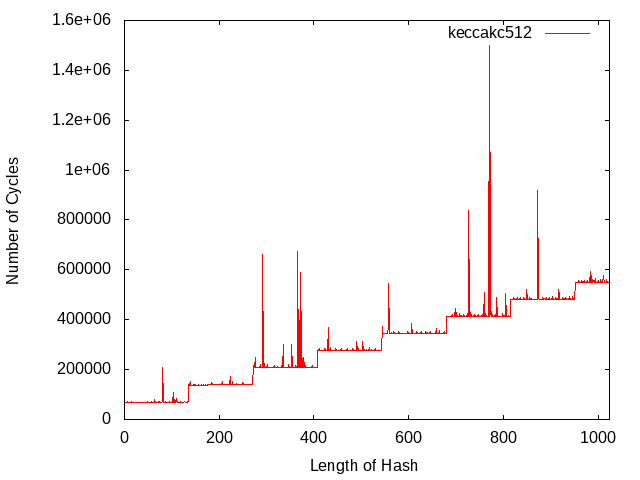
\includegraphics[scale=0.5]{images/keccakc512.png} 
        \caption{Keccak[r=1088,c=512,nr=24] with 256-bit output}
    \end{center}
\end{figure}

The algorithm selected to benchmark Keccakc512 was compact8 which had been
compiled with \texttt{gcc -mcpu=strongarm1100 -O3 -fomit-frame-pointer} on GCC
version 4.4.5. This variant of Keccak has the parameters $r=1088,c=512,n_r=24$.

Interestingly, this implementation is not what the other implementations had
been compiled with, though it is a similar implementation.

The prediction regarding the stair stepped pattern as well as the period between
the steps being proportional to the bit rate however was upheld regardless of
the differences in version. This is because the amount of work being done is
somewhat inherent in the algorithm, and these implementations are very similar.


\subsubsection{keccakc768}
\begin{figure}[H]
    \begin{center}
        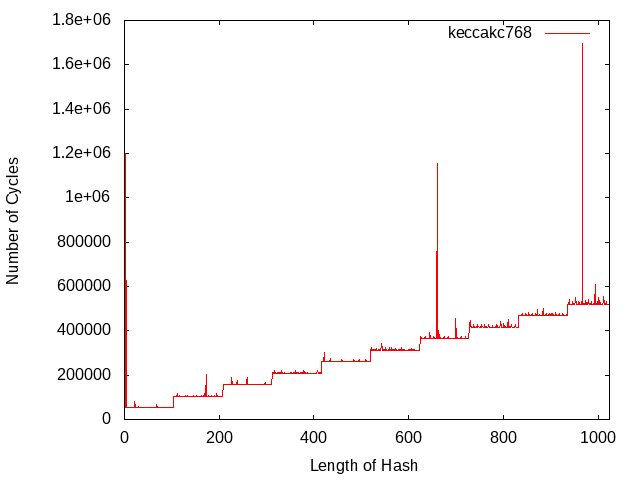
\includegraphics[scale=0.5]{images/keccakc768.png} 
        \caption{Keccak[r=832,c=768,nr=24] with 384-bit output}
    \end{center}
\end{figure}

The algorithm selected to benchmark Keccakc768 was compact which had been
compiled with \texttt{gcc -mcpu=strongarm1100 -O -fomit-frame-pointer} on GCC
version 4.4.5. This variant of Keccak has the parameters $r=832,c=768,n_r=24$.

A return to implementations of Keccak being compiled with compact on this board,
this run exhibited the exact same properties that we have been seeing before.
The stepped pattern is now shorter still because of the direct correlation with
the bit rate $r$. This performance property is a property of the algorithm
family.


\subsubsection{keccakc1024}
\begin{figure}[H]
    \begin{center}
        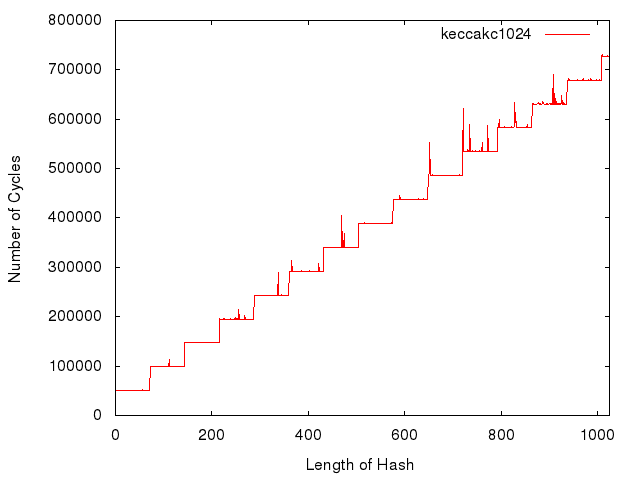
\includegraphics[scale=0.5]{images/keccakc1024.png} 
        \caption{Keccak[r=576,c=1024,nr=24] with 512-bit output}
    \end{center}
\end{figure}

The algorithm selected to benchmark Keccakc1024 was compact which had been
compiled with \texttt{gcc -mcpu=cortex-a8 -mfloat-abi=softfp -mfpu=neon -O
-fomit-frame-pointer} on GCC version 4.4.5. This variant of Keccak has the
parameters $r=576,c=1024,nr=24$.

The version of Keccak with the shortest bit rate that we tested, and it still
upholds the prediction that the bit rate is directly correlated with the period
between the steps. In this variant, the jumps in cycle count is very rapid,
causing the algorithm to consume a much higher number of clock cycles by the
time it has finished compared to the lower capacity variants of Keccak.
